Для разработки и запуска шаблонов необходима оперционная система Linux. Без неё не возможна работа с "ЧАС ЕГЭ".

Вместо установки полноценной операционной системы на компьютер, мы выбрали более удобный вариант. Мы предпочли скачать программу VirtualBox и поставить на неё Linux. Далее идёт описание процесса установки и запуска Виртуальной машины.

\quad 1.\quad Перейходим по ссылке https://www.virtualbox.org. Нажимаем кнопку «Download», выбираем «Windows hosts» и устанавливаем VirtualBox. 

\begin{figure}[h]	
		\centering
		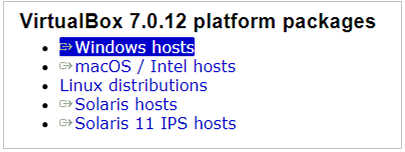
\includegraphics[width=0.9\linewidth]{VM/1.png}
\caption{«Windows hosts».}
\label{ris:image}
\end{figure}

\quad 2.\quad Далее, для того чтобы любая виртуальная машина могла работать, необходимо включить виртуализацию. В данном случае, мы имеем дело с Windows 11. Чтобы проверить включена ли на ней виртуализация, открываем диспетчер задач и переходим в раздел «Производительность». Диспетчер задач можно открыть, нажав по панели задач правой кнопкой мыши и выбрав соответсвующий пункт. Или можно зажать клавиши Ctrl+Alt+Del, и в открывшемся меню выбрать диспетчер задач.

\begin{figure}[h]
		\centering
		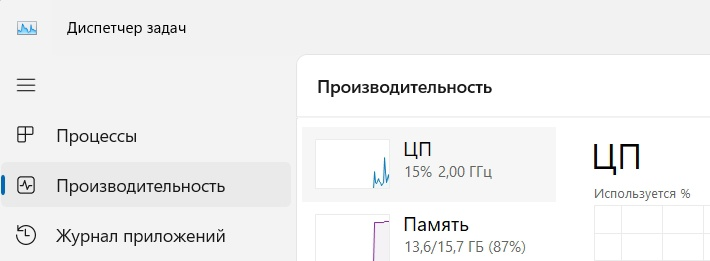
\includegraphics[width=0.9\linewidth]{VM/Disp.jpg}
\caption{Диспетчер задач. Производительность.}
\label{ris:image}
\end{figure}


 Открываем окно диспетчера задач на весь экран и внизу увидим, включена ли виртуализация.

\begin{figure}[h]
		\centering
		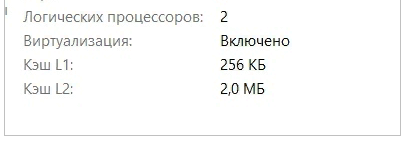
\includegraphics[width=0.9\linewidth]{VM/2.png}
\caption{Виртуализация.}
\label{ris:image}
\end{figure}

\quad Если виртуализация выключена, то необходимо войти в BIOS. Для этого нужно нажать на кнопку «Перезагрузить компьютер», и, как только он начинает запускаться, зажать клавишу «Esc» или начать нажимать много раз на клавишу delete, обычно именно эта клавиша используется на стационарных компьютерах для запуска BIOS, пока не запустится «Startup menu». На ноутбуках чаще всего для входа в BIOS используется клавиша F2 (иногда в сочетании с Fn), но встречаются и другие клавиши или их комбинации, зависящие от производителя (Ctrl + Alt + Ins, Ctrl + Alt + F3, Ctrl + Alt + S и др.). Чтобы открыть BIOS надо нажать клавишу «F10» и перейти в «System Configuration», нажав два раза на кнопку со стрелкой вправо. Затем, с помощью стрелки вниз, перейти к «Virtualization Technology» и нажать клавишу «Enter». Далее нужно выбрать «Enable» и снова нажать «Enter». Затем снова нажать «F10» и выбрать «Yes», после чего компьютер перезагрузится уже с включённой виртуализацией.


\begin{figure}[h]
		\centering
		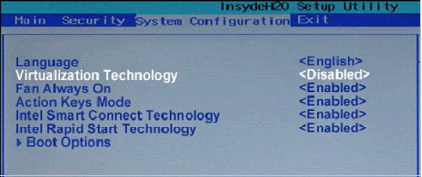
\includegraphics[width=0.9\linewidth]{VM/3.png}
\caption{BIOS. «Virtualization Technology».}
\label{ris:image}
\end{figure}

3. Скачиваем Ubuntu с официального сайта по ссылке: https://ubuntu.com/download/desktop. В нашем случае, мы воспользовались версией Ubuntu 22.04.3. Затем открываем VirtualBox и нажимаем кнопку «Создать». Заполняя все поля, необходимо потянуть ползунок вправо, чтобы увеличить объем оперативной памяти, который будет использоваться виртуальной машиной. Для работы с Ubuntu минимальный размер объёма памяти должен быть не менее 2 гигабайт, иначе она не запустится. В остальном можно принять все установки по умолчанию. После создания, необходимо нажать на кнопку «Настройки», далее «Носители», у надписи «Контроллер: IDE» нажать на значок диска с плюсом. 

\begin{figure}[h]
		\centering
		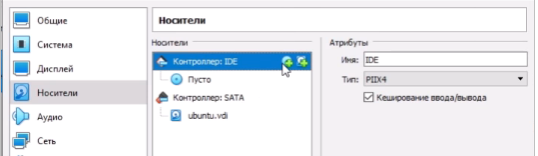
\includegraphics[width=0.65\linewidth]{VM/4.png}
\caption{Настройки. Носители.}
\label{ris:image}

\end{figure}

\quad Затем «Добавить» и выбрать скачанный ранее файл с Ubuntu. Далее нажимаем кнопку «Запустить». После запуска, выбираем язык, нажимаем «установить Ubuntu», заполняем все поля и выбираем параметры.

\begin{figure}[h]
		\centering
		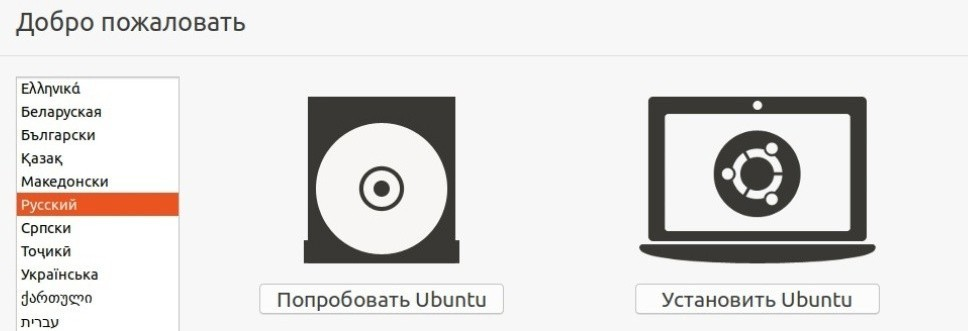
\includegraphics[width=0.65\linewidth]{VM/ubu.jpg}
\caption{Ubuntu.}
\label{ris:image}

\end{figure}

И наконец видим интерфейс Linux.

\begin{figure}[h]
		\centering
		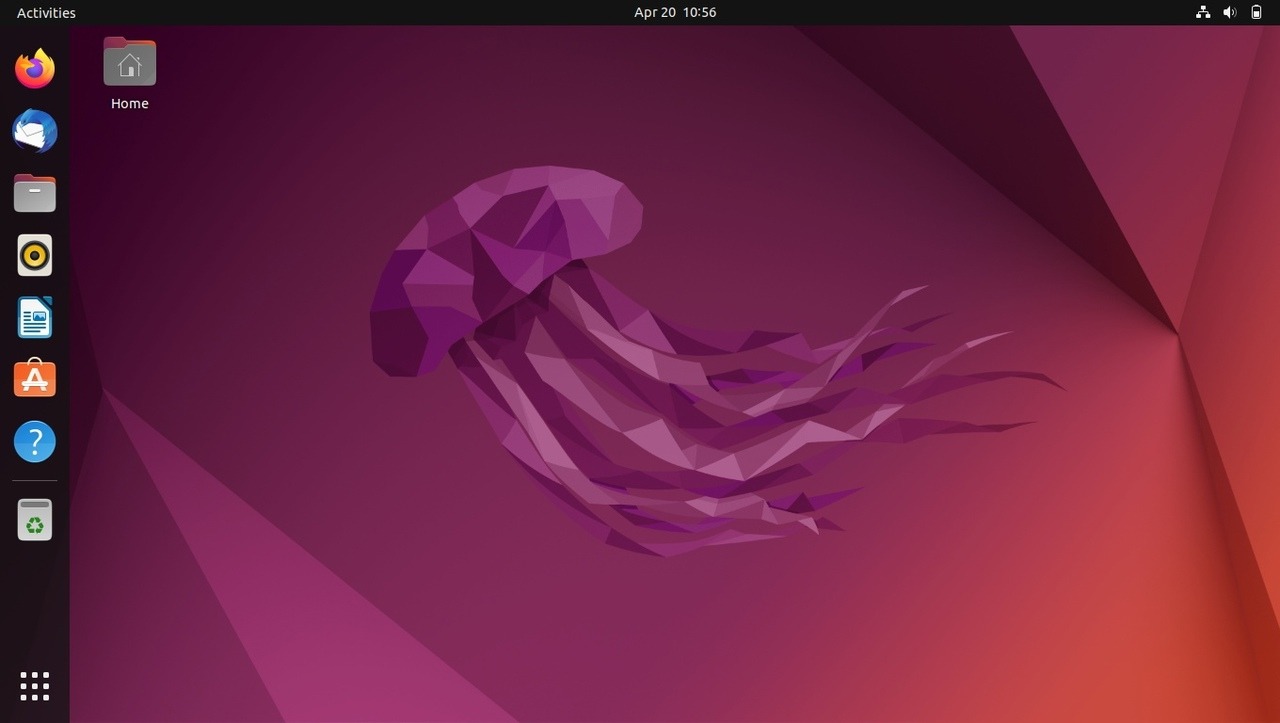
\includegraphics[width=0.5\linewidth]{VM/lin.jpg}
\caption{Linux.}
\label{ris:image}

\end{figure}


